\documentclass{article}
\usepackage[utf8]{vietnam}
\usepackage{graphicx}

%%%%%%%%%%%%%%%%%%%%%%%%%%%%%%%%%%%%%%%%%%%%%%%%%%%%%%%
\begin{document}
%%%%%%%%%%%%%%%%%%%%%%%%%%%%%%%%%%%%%%%%%%%%%%%%%%%%%%%
\section{Tuần 1}



\subsection{Video 1}

\subsubsection{Hướng dẫn}
\paragraph{Sắp xếp dữ liệu}

\subparagraph{Sắp xếp dữ liệu theo 1 tiêu chí}
\begin{figure}[h]
    \centering
    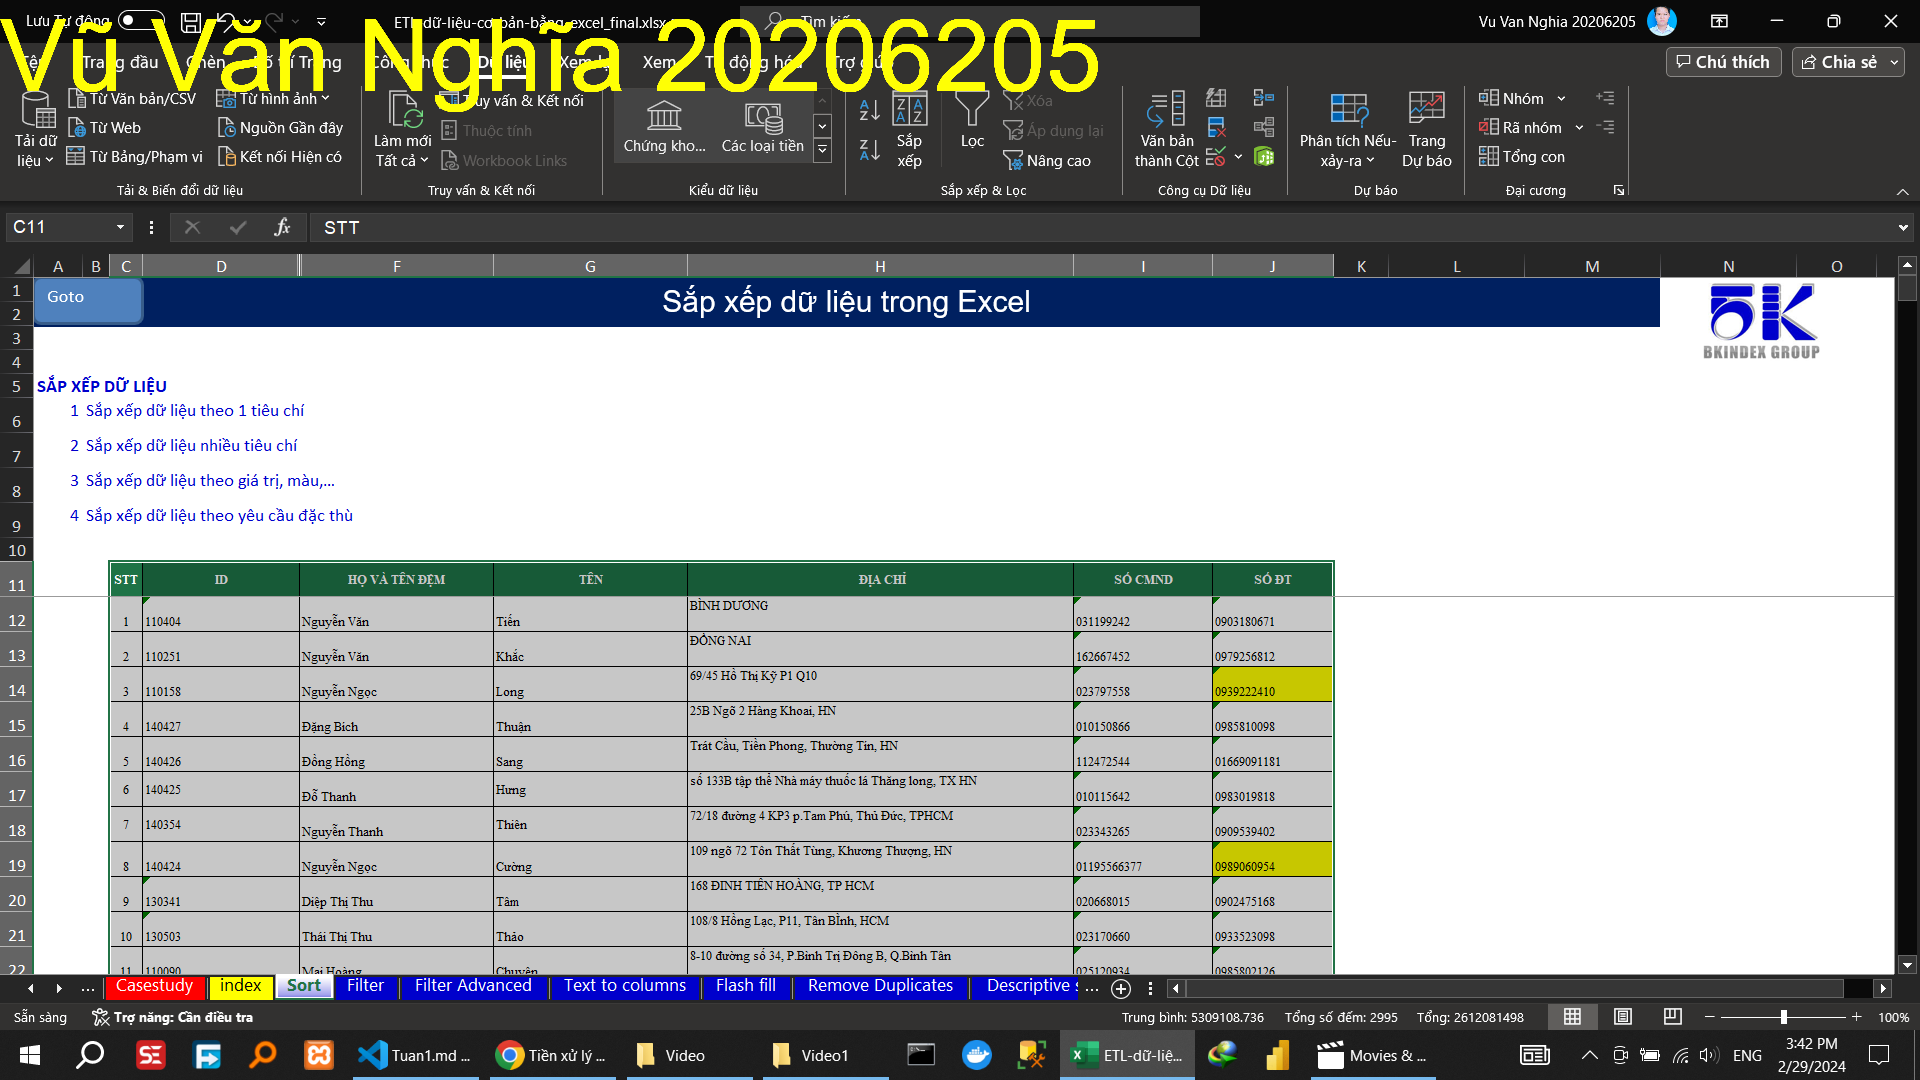
\includegraphics[scale = 0.15]{Video1/HuongDan/1.png}
    \caption{Sắp xếp dữ liệu theo 1 tiêu chí là số thứ tự}
\end{figure}

\subparagraph{Sắp xếp dữ liệu theo nhiều tiêu chí}
\begin{figure}[h]
    \centering
    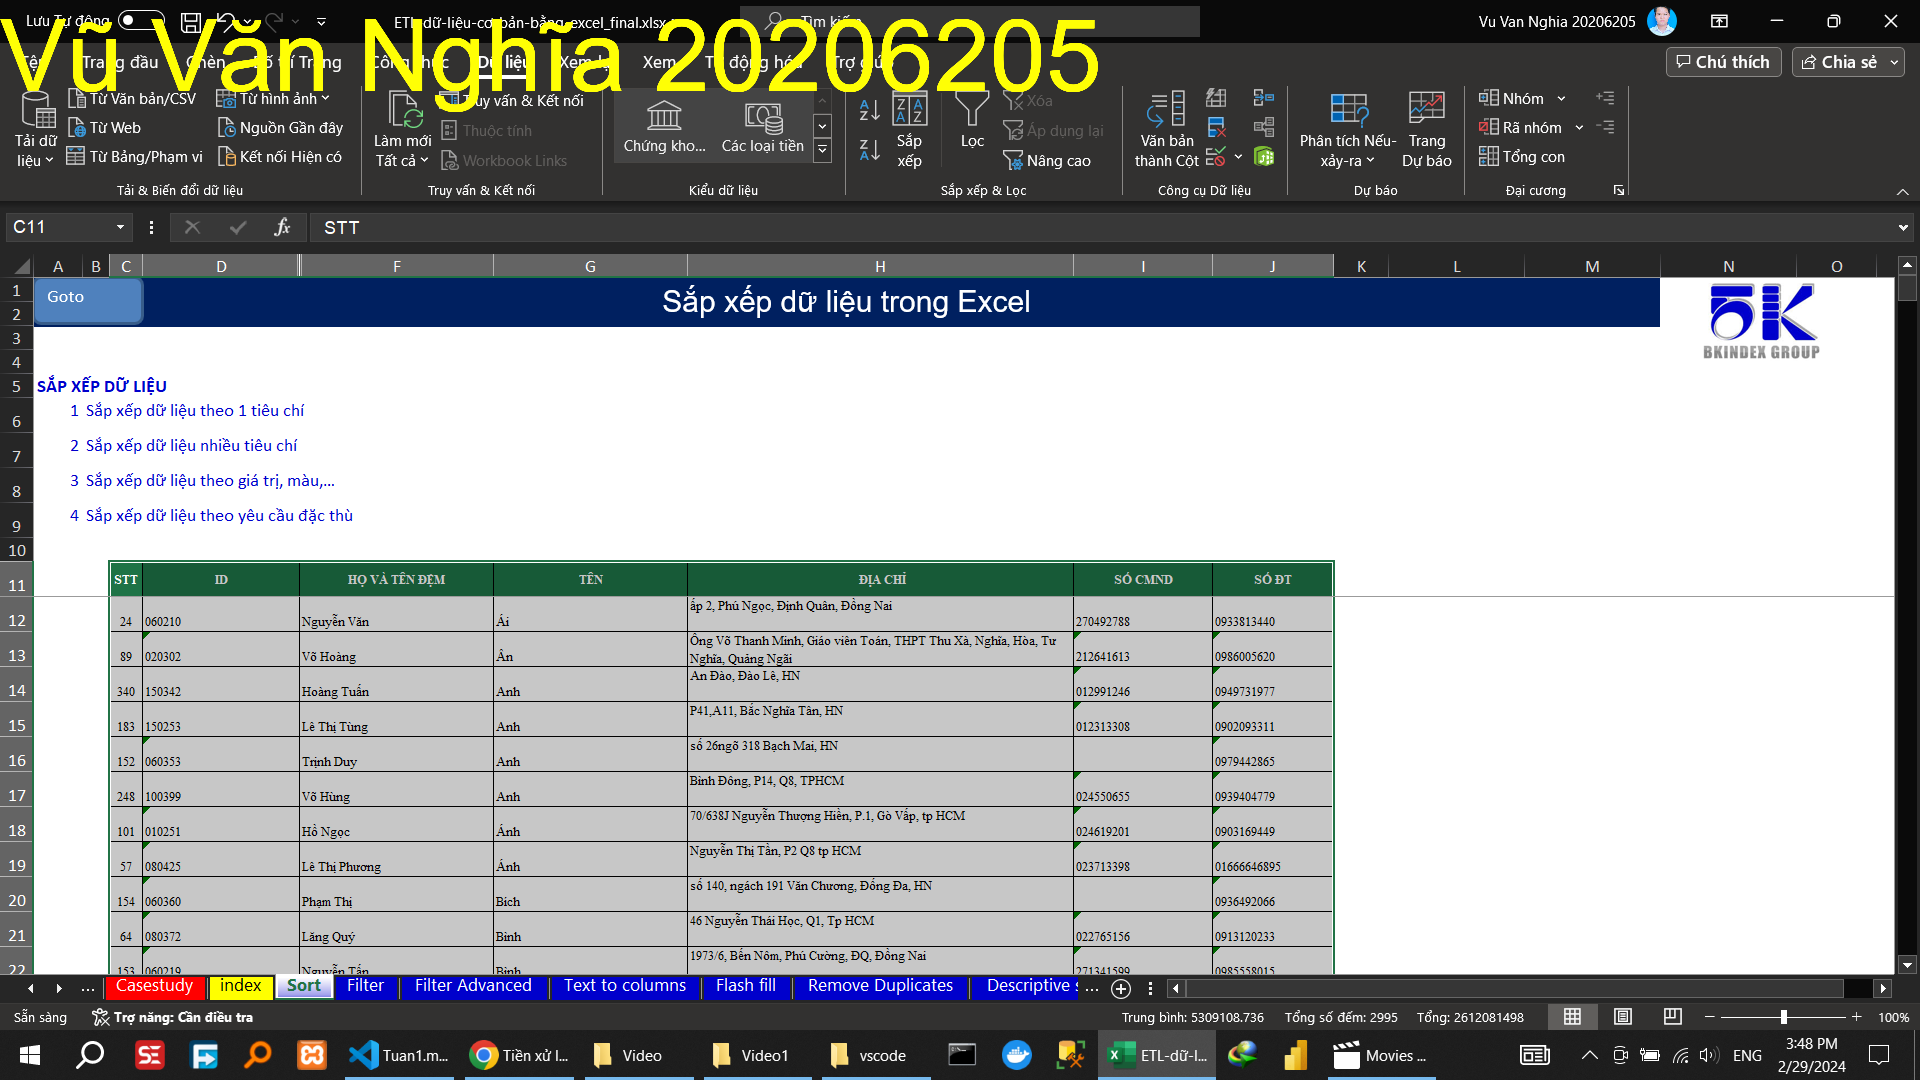
\includegraphics[scale = 0.15]{Video1/HuongDan/2.png}
    \caption{Sắp xếp dữ liệu theo  nhiều tiêu chí họ và tên đệm}
\end{figure}

\subparagraph{Sắp xếp dữ liệu theo giá trị, màu,\dots}
\begin{figure}[h]
    \centering
    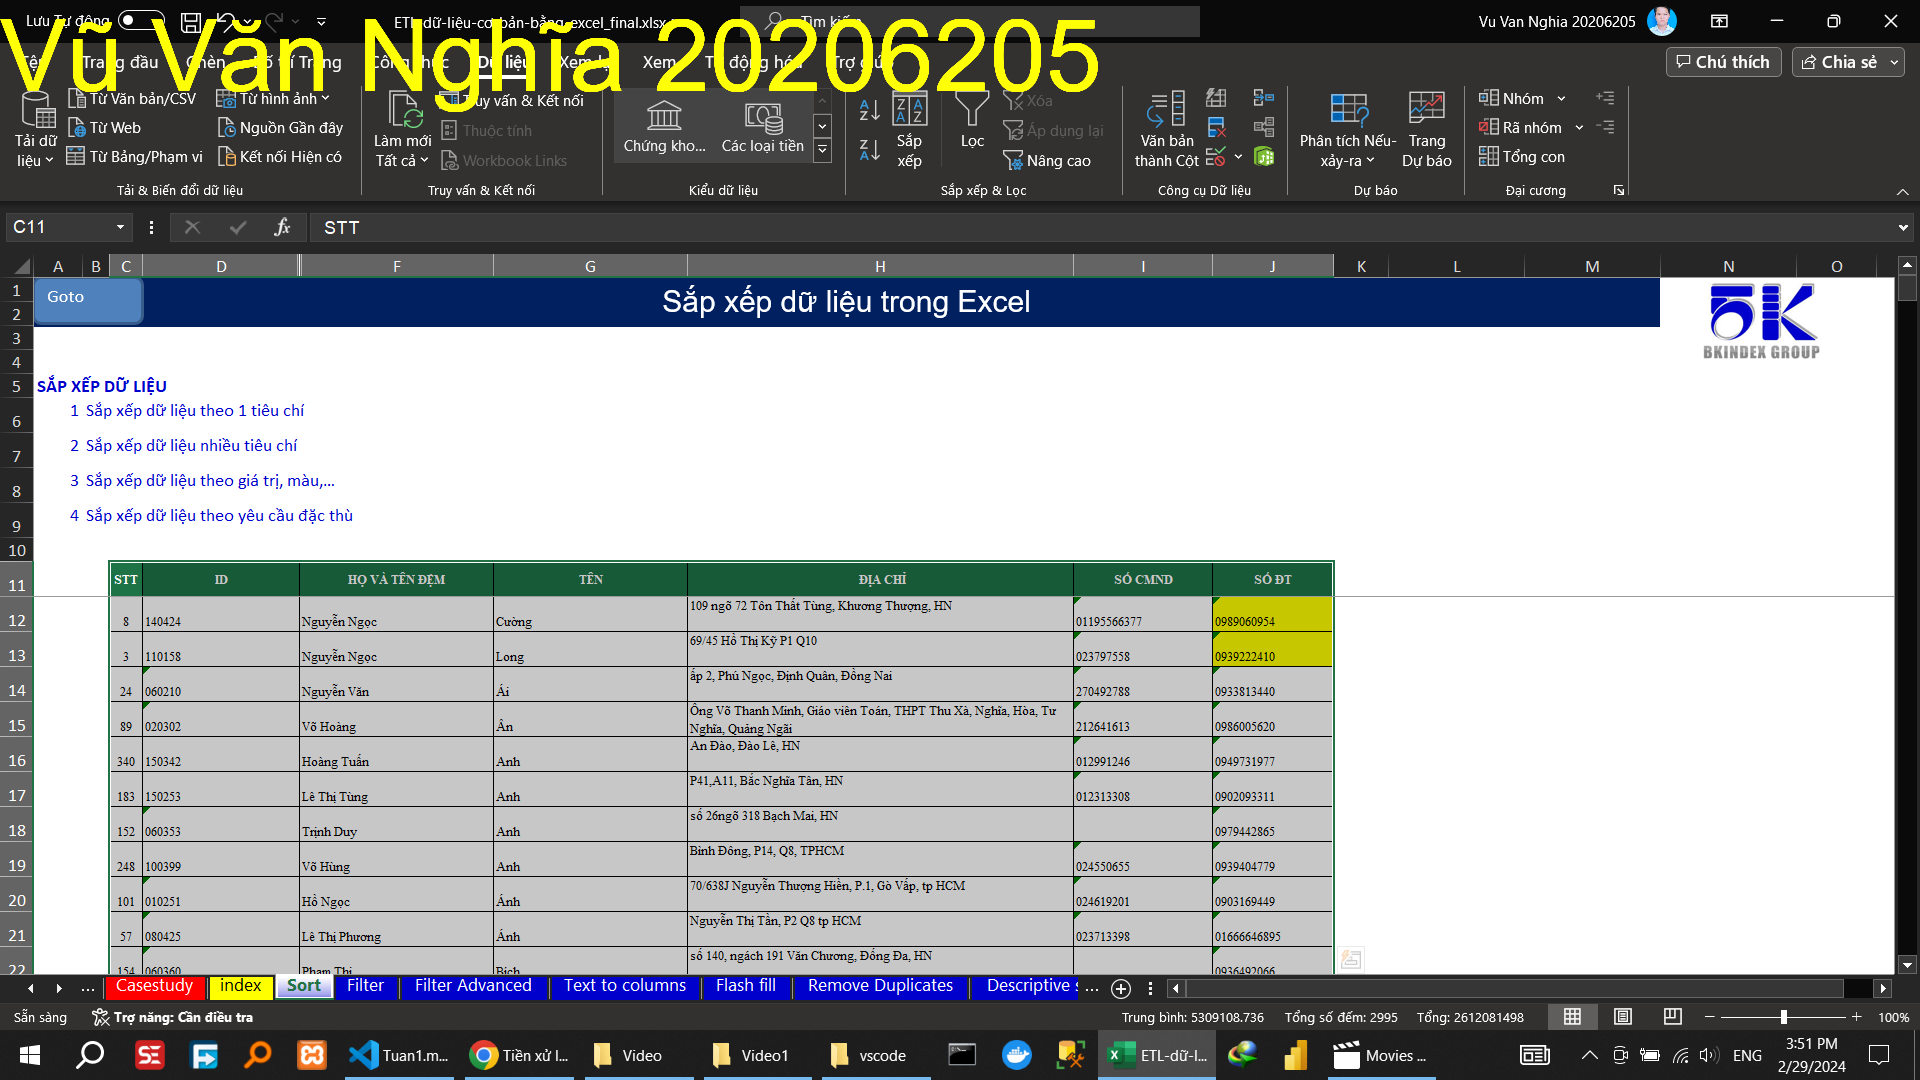
\includegraphics[scale = 0.15]{Video1/HuongDan/3.png}
    \caption{Sắp xếp dữ liệu theo  giá trị, màu,\dots của số điện thoại}
\end{figure}


% #### 

% ##### 

% ![Sắp xếp theo STT](HuongDan/11.png)

% ##### 

% ![xxxxxxxxxxxxxxxxxxxxxxxxxxx](HuongDan/image.png)

% ##### 

% ![xxxxxxxxxxxxxxxxxxxxxxxxxxx](HuongDan/image-1.png)




\subsubsection{Thực hành}



\subsection{Video 2}
\subsubsection{Hướng dẫn}

\subsubsection{Thực hành}




\subsection{Video 3}
\subsubsection{Hướng dẫn}

\subsubsection{Thực hành}




\subsection{Video 4}
\subsubsection{Hướng dẫn}

\subsubsection{Thực hành}




\subsection{Video 5}
\subsubsection{Hướng dẫn}

\subsubsection{Thực hành}




\subsection{Video 6}
\subsubsection{Hướng dẫn}

\subsubsection{Thực hành}




\subsection{Video 7}
\subsubsection{Hướng dẫn}

\subsubsection{Thực hành}




\subsection{Video 8}
\subsubsection{Hướng dẫn}

\subsubsection{Thực hành}








%%%%%%%%%%%%%%%%%%%%%%%%%%%%%%%%%%%%%%%%%%%%%%%%%%%%%%%
\end{document}
%%%%%%%%%%%%%%%%%%%%%%%%%%%%%%%%%%%%%%%%%%%%%%%%%%%%%%%





\begin{figure}[h]
    \centering
    \includegraphics[width=0.5\textwidth]{example-image-a}
    \caption{Ví dụ về hình ảnh}
    \label{fig:example}
\end{figure}